\section{Photometric ETC}
\label{sec:photometry}

\subsection{Signal and noise budget}
\label{sec:noise}

For a circular aperture of radius $r$ containing
$N_{\rm pix} = \pi r^2 / p^2$ pixels ($p$ = plate scale per pixel), the
extracted source signal is $S = \dot S\,\mathrm{EE}(r)\,t_{\rm exp}$, the sky
signal is $B = \dot B\,\pi r^2\, t_{\rm exp}$ from the observed surface
brightness of Sect.~\ref{sec:sky}, and the dark charge is
$D = \dot d\,N_{\rm pix}\,t_{\rm exp}$. The S/N is the CCD equation extended
with the multiplicative and quantization terms:
\begin{equation}
  \mathrm{S/N} \;=\;
  \frac{S}{\sqrt{\;S + B + D + N_{\rm pix}\,\sigma_R^2
        + \big(S\,\sigma_{\rm scint}/I\big)^2
        + N_{\rm pix}\, g^2/12\;}} ,
  \label{eq:snr}
\end{equation}
with the scintillation fraction of Eq.~(\ref{eq:scint}) and the ADC
quantization variance $g^2/12$ per pixel \citep{janesick2001}. Flat-field
residuals are deliberately not modelled. The inverse problem --- the exposure
that reaches a requested S/N --- is solved in closed form from the quadratic
obtained from Eq.~(\ref{eq:snr}) with the Poisson terms proportional to $t$.

\begin{table}
\centering
\caption{Noise terms and their scalings.}
\label{tab:noise}
\begin{tabular}{llll}
\toprule
Term & Variance [e$^{-2}$] & Scaling & Reference \\
\midrule
Source shot     & $S$ & $\propto t$ & --- \\
Sky shot        & $B$ & $\propto t\,r^2$ & Sect.~\ref{sec:sky} \\
Dark            & $D$ & $\propto t\,N_{\rm pix}$ & --- \\
Read            & $N_{\rm pix}\sigma_R^2$ & per frame & --- \\
Scintillation   & $(S\,\sigma_{\rm scint}/I)^2$ & $\propto t^{1}$\,$^{a}$ &
\citet{young1967,osborn2015} \\
Quantization    & $N_{\rm pix}\,g^2/12$ & per frame & \citet{janesick2001} \\
\bottomrule
\end{tabular}

\smallskip
{\footnotesize $^{a}$ $S \propto t$ while $\sigma_{\rm scint}/I \propto
t^{-1/2}$, so the S/N ceiling $I/\sigma_{\rm scint} \propto \sqrt{t}$.}
\end{table}

\subsection{Saturation}

Saturation is evaluated on the brightest pixel of the \emph{unextracted}
image: the PSF central-pixel fraction (Sect.~\ref{sec:psf}) times the total
source charge, plus the per-pixel sky and dark. The peak is compared with
both the full well and the ADC ceiling $g\,(2^{N_{\rm bit}}-1)$, and the flag
distinguishes \code{FULL\_WELL}, \code{ADC}, \code{BOTH} and \code{NONE};
the maximum unsaturated single-frame exposure is reported at every time
sample.

\subsection{Extended sources}
\label{sec:extended}

Galaxies, nebulae and planets are modelled as uniform surface brightness over
a stated angular area $\Omega$: the entered magnitude remains the
\emph{integrated} magnitude, so the mean surface rate is $\dot S/\Omega$ per
arcsec$^2$. The aperture then captures the area fraction
$\min(\pi r^2/\Omega,\,1)$ with no PSF concentration loss, and the peak pixel
holds $\dot S\,p^2/\Omega$ --- the appropriate saturation criterion for a
resolved source. The approximation is stated to be valid when the source is
much larger than the seeing disc, where PSF blur merely redistributes light
across the source edge.

\begin{figure}
  \centering
  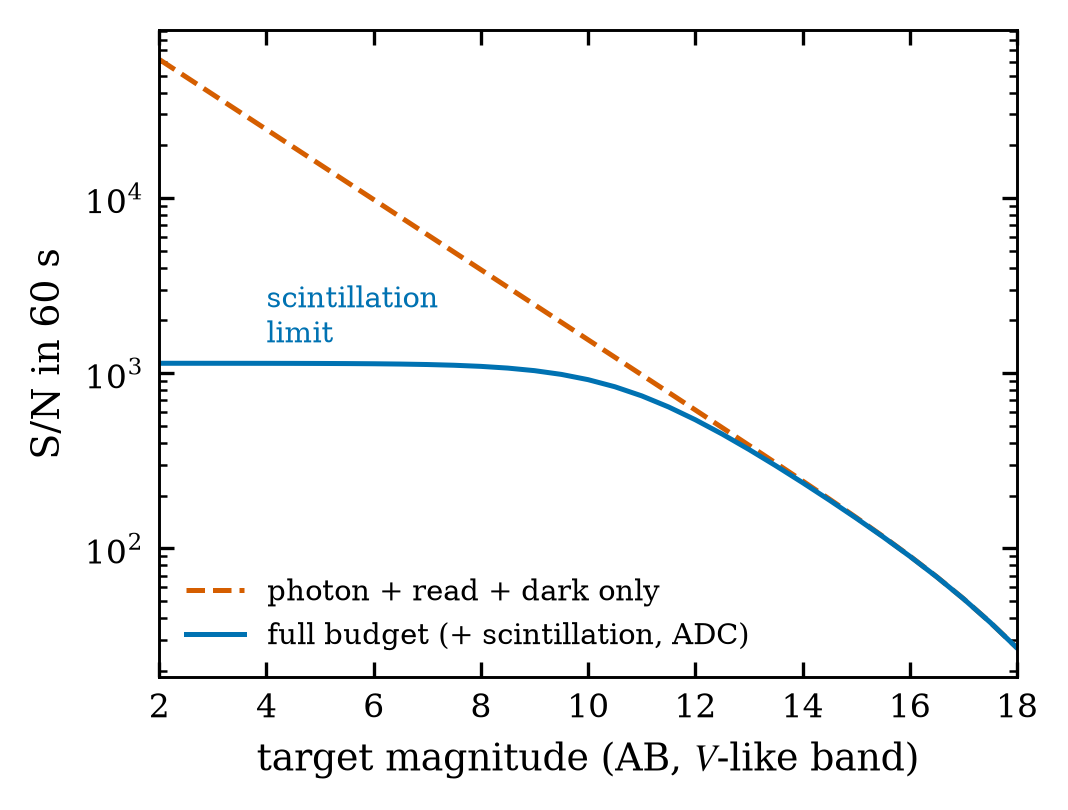
\includegraphics[width=0.62\textwidth]{figures/fig_06_snr_budget.png}
  \caption{Broad-band S/N in \SI{60}{s} for the 358-mm reference
  configuration, computed by the released code. The full budget
  (solid) saturates at the scintillation ceiling
  $\simeq 1.2\times10^{3}$; a Poisson-only model (dashed) overestimates
  bright-star performance by more than an order of magnitude.}
  \label{fig:snrbudget}
\end{figure}
